\documentclass[10pt, a4paper, twocolumn]{article} % 10pt font size (11 and 12 also possible), A4 paper (letterpaper for US letter) and two column layout (remove for one column)

%%%%%%%%%%%%%%%%%%%%%%%%%%%%%%%%%%%%%%%%%
% Wenneker Article
% Structure Specification File
% Version 1.0 (28/2/17)
%
% This file originates from:
% http://www.LaTeXTemplates.com
%
% Authors:
% Frits Wenneker
% Vel (vel@LaTeXTemplates.com)
%
% License:
% CC BY-NC-SA 3.0 (http://creativecommons.org/licenses/by-nc-sa/3.0/)
%
%%%%%%%%%%%%%%%%%%%%%%%%%%%%%%%%%%%%%%%%%

%----------------------------------------------------------------------------------------
%	PACKAGES AND OTHER DOCUMENT CONFIGURATIONS
%----------------------------------------------------------------------------------------

\usepackage[english]{babel} % English language hyphenation

\usepackage{microtype} % Better typography

\usepackage{amsmath,amsfonts,amsthm} % Math packages for equations

\usepackage[svgnames]{xcolor} % Enabling colors by their 'svgnames'

\usepackage[hang, small, labelfont=bf, up, textfont=it]{caption} % Custom captions under/above tables and figures

\usepackage{booktabs} % Horizontal rules in tables

\usepackage{lastpage} % Used to determine the number of pages in the document (for "Page X of Total")

\usepackage{graphicx} % Required for adding images

\usepackage{enumitem} % Required for customising lists
\setlist{noitemsep} % Remove spacing between bullet/numbered list elements

\usepackage{threeparttable}

\usepackage{sectsty} % Enables custom section titles
\allsectionsfont{\usefont{OT1}{phv}{b}{n}} % Change the font of all section commands (Helvetica)

%----------------------------------------------------------------------------------------
%	MARGINS AND SPACING
%----------------------------------------------------------------------------------------

\usepackage{geometry} % Required for adjusting page dimensions

\geometry{
	top=1cm, % Top margin
	bottom=1.5cm, % Bottom margin
	left=2cm, % Left margin
	right=2cm, % Right margin
	includehead, % Include space for a header
	includefoot, % Include space for a footer
	%showframe, % Uncomment to show how the type block is set on the page
}

\setlength{\columnsep}{7mm} % Column separation width

%----------------------------------------------------------------------------------------
%	FONTS
%----------------------------------------------------------------------------------------

\usepackage[T1]{fontenc} % Output font encoding for international characters
\usepackage[utf8]{inputenc} % Required for inputting international characters

\usepackage{XCharter} % Use the XCharter font

%----------------------------------------------------------------------------------------
%	HEADERS AND FOOTERS
%----------------------------------------------------------------------------------------

\usepackage{fancyhdr} % Needed to define custom headers/footers
\pagestyle{fancy} % Enables the custom headers/footers

\renewcommand{\headrulewidth}{0.0pt} % No header rule
\renewcommand{\footrulewidth}{0.4pt} % Thin footer rule

\renewcommand{\sectionmark}[1]{\markboth{#1}{}} % Removes the section number from the header when \leftmark is used

%\nouppercase\leftmark % Add this to one of the lines below if you want a section title in the header/footer

% Headers
\lhead{} % Left header
\chead{\textit{\thetitle}} % Center header - currently printing the article title
\rhead{} % Right header

% Footers
\lfoot{} % Left footer
\cfoot{} % Center footer
\rfoot{\footnotesize Page \thepage\ of \pageref{LastPage}} % Right footer, "Page 1 of 2"

\fancypagestyle{firstpage}{ % Page style for the first page with the title
	\fancyhf{}
	\renewcommand{\footrulewidth}{0pt} % Suppress footer rule
}

%----------------------------------------------------------------------------------------
%	TITLE SECTION
%----------------------------------------------------------------------------------------

\newcommand{\authorstyle}[1]{{\large\usefont{OT1}{phv}{b}{n}\color{DarkRed}#1}} % Authors style (Helvetica)

\newcommand{\institution}[1]{{\footnotesize\usefont{OT1}{phv}{m}{sl}\color{Black}#1}} % Institutions style (Helvetica)

\usepackage{titling} % Allows custom title configuration

\newcommand{\HorRule}{\color{DarkGoldenrod}\rule{\linewidth}{1pt}} % Defines the gold horizontal rule around the title

\pretitle{
	\vspace{-30pt} % Move the entire title section up
	\HorRule\vspace{10pt} % Horizontal rule before the title
	\fontsize{32}{36}\usefont{OT1}{phv}{b}{n}\selectfont % Helvetica
	\color{DarkRed} % Text colour for the title and author(s)
}

\posttitle{\par\vskip 15pt} % Whitespace under the title

\preauthor{} % Anything that will appear before \author is printed

\postauthor{ % Anything that will appear after \author is printed
	\vspace{10pt} % Space before the rule
	\par\HorRule % Horizontal rule after the title
	\vspace{20pt} % Space after the title section
}

%----------------------------------------------------------------------------------------
%	ABSTRACT
%----------------------------------------------------------------------------------------

\usepackage{lettrine} % Package to accentuate the first letter of the text (lettrine)
\usepackage{fix-cm}	% Fixes the height of the lettrine

\newcommand{\initial}[1]{ % Defines the command and style for the lettrine
	\lettrine[lines=3,findent=4pt,nindent=0pt]{% Lettrine takes up 3 lines, the text to the right of it is indented 4pt and further indenting of lines 2+ is stopped
		\color{DarkGoldenrod}% Lettrine colour
		{#1}% The letter
	}{}%
}

\usepackage{xstring} % Required for string manipulation

\newcommand{\lettrineabstract}[1]{
	\StrLeft{#1}{1}[\firstletter] % Capture the first letter of the abstract for the lettrine
	\initial{\firstletter}\textbf{\StrGobbleLeft{#1}{1}} % Print the abstract with the first letter as a lettrine and the rest in bold
}

%----------------------------------------------------------------------------------------
%	BIBLIOGRAPHY
%----------------------------------------------------------------------------------------

\usepackage[backend=bibtex,style=authoryear,natbib=true]{biblatex} % Use the bibtex backend with the authoryear citation style (which resembles APA)

\addbibresource{biblio.bib} % The filename of the bibliography

\usepackage[autostyle=true]{csquotes} % Required to generate language-dependent quotes in the bibliography


%----------------------------------------------------------------------------------------
%	ALESSANDRO'S ADDITIONS
%----------------------------------------------------------------------------------------

\newcommand{\ie}{\textit{i.e.,} }
\newcommand{\eg}{\textit{e.g.,} }
\newcommand{\wrt}{\textit{w.r.t.\ }}

\newcommand{\todobox}[3]{%
	\colorbox{#1}{\textcolor{white}{\sffamily\bfseries\scriptsize #2}}%
	~\textcolor{blue}{#3} %
	\textcolor{#1}{$\triangleleft$}%
}
\newcommand{\todo}[1]{\todobox{red}{TODO}{#1}}
\newcommand{\feedback}[1]{\todobox{orange}{OK?}{#1}}
\newcommand{\done}[1]{\todobox{blue}{DONE}{#1}}
\newcommand{\rationale}[1]{\todobox{ForestGreen}{RATIONALE}{#1}}

\usepackage{balance}
\usepackage{subcaption} % Specifies the document structure and loads requires packages

%----------------------------------------------------------------------------------------
%	ARTICLE INFORMATION
%----------------------------------------------------------------------------------------

\title{On the security of collective \\ remote attestation protocols: the case study of SANA} % The article title

\author{
	\authorstyle{Alessandro Rizzo and Davide Maria Lazzaro} % Authors
	\newline\newline % Space before institutions
	\textsuperscript{1}\institution{Università degli studi di Padova, Padova, Italy}\\ % Institution 1
}

\date{\today}

%----------------------------------------------------------------------------------------

\begin{document}

\maketitle % Print the title

\thispagestyle{firstpage} % Apply the page style for the first page (no headers and footers)

%Se avete abstract, abilitate questo
\lettrineabstract{Software integrity for IOT devices is an open challenge in CyberSecurity. These devices have particular constraints in term of memory and computational capabilities. SANA offers to solve this problem using an Optimistic Aggregated Signature scheme that lower the computational and memory cost for the attestation. In this paper we implement SANA using a modern ECC implementation called ''bn128'' in order to verify the claims of the original paper and review criticalities in the protocol. We show the performances of our implementation compared to the original ones and discuss if and how this protocol can be efficiently applied in the scneario of IOT devices.}


\section{Introduction}

The Internet of Things (IoT) paradigm promises to interconnect the world and
change the way data is collected and processed.
This revolution is largely built on the establishment of large networks of small 
devices that autonomously exchange data.
Typically, these devices have low computational capabilities and process
sensible data.
As a consequence, these networks attract the attention of malicious entities
that attempt to exploit the poor security standards usually employed in such
environments.

Remote Attestation (RA) has been suggested as a potential solution to mitigate the
security concerns.
It allows a remote entity (\ie Verifier) to validate the integrity of
the software of a local device (\ie Prover).
This process usually makes use of a signed hash value of the Prover’s software, 
generated by dedicated hardware.
To deal with scalability issues, Collective Remote Attestation (CRA) has 
been proposed as an adaptation of classical RA to check the status of a network 
in a decentralized fashion.

SANA(~\cite{sana}) is a CRA scheme that promises to inspect the overall
status of an IoT network with a single and efficient operation.
\todo{add explanation on tree propagation.}
It does so by introducing a signature scheme called Optimistic Aggregated
Signature (OAS) which allows the aggregation of the signatures coming from
different devices.
The aggregated signature is smaller than the naive one (\ie list of appended
signatures) and makes the verification cost dependant only on the number of
compromised devices.
SANA comes with estimations about its memory, communication, and computational costs. But the formulas neglect specifying some variables that prove to be decisive to determine these estimations.
We chose to implement the protocol using an ECC algorithm based on Ethereum to handle the signing and verification phases of the protocol, then we analyzed the results to prove the claims that were given in the SANA paper and at last make some considerations about the criticality of this protocol.

In this article we verify the security claims made in SANA's paper.
In particular we focus on checking the overall cost for running the protocol
\todo{and the soundness of its propagation process (if done)}.
\todo{list the results obtained.}
\section{Premises}

\begin{figure*}
	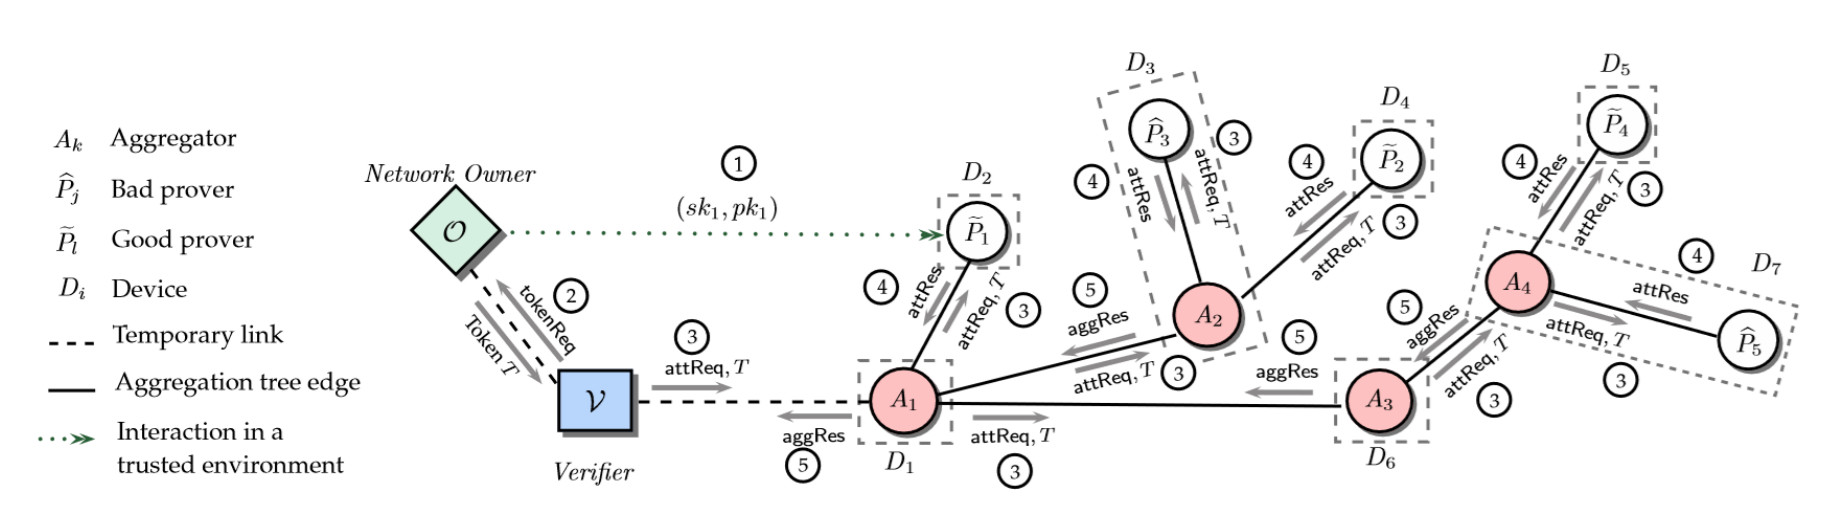
\includegraphics[width=0.9\linewidth]{Images/SANA_general.png} % Figure image
	\caption{Schematic of SANA propagation tree} % Figure caption
\end{figure*}

\subsection{Elliptic curve cryptography}
\todo{here just introduce ECC in general}
Elliptic Curve Cryptography (ECC) \todo{add citation.} is a public key
cryptographic method based on the algebraic structure of elliptic curves over
finite fields.
ECC security is based on the intractability of the elliptic
curve discrete logarithm problem.
In particular, it depends on the simplicity of computing a point multiplication 
on the curve as opposed to the intractability of computing the scalar multiplicand
given the original point and the result.
All this operations are performed with respect to the finite field the curve is associated with.

\subsection{SANA attestation protocol}
\todo{here introduce SANA propagation and how ECC is integrated in it.}
In SANA the remote attestation process starts from the verifier that sends a request to the Owner that generates a Token and propagates it to the Verifier (containing a challenge that will be proposed to the other nodes in order to certify the authenticity of the attestation request). The Verifier checks the signature and, if it has a positive result, stores the token. \\The Verifier then
the challenge to the closest Aggregator in the propagation tree, this node proceeds to propagate the challenge to its neighbours being other Aggregator
or Provers. The latter then sign a message according to their software configuration being legit or compromised. The signature travel back to the Aggregator
that creates the aggregated signature of its neighbours. Lastly the Verifier checks the aggregated signature of all the tree and determines which devices
can be trusted and which are compromised.\\
For implementing this protocol we chose an elliptic-curve implementation used in Ethereum and called ''bn128'' as it uses a Barreto-Naehrig curve and it's said to offer 128 bits security.
In SANA, the ECC is used to generate public keys that belong to a multiplicative
group that is composed by points on the curve we have chosen for the cryptrographic system.
After that all the signatures are generated by a random oracle as points belonging to the curve. We then use a fancy property of Elliptic curve to perform a bilinear function (called also pairing) on the signature received and a reconstruction of what should be the signature to check if it's authentic in a computationally efficient way.
\section{Implementation details}


This SANA implementation uses ''bn128'', an ECC implementation that uses an already existing curve belonging to Barreto-Naherig set of curves.
This implementation uses the Barreto-Naehrig curve on a finite field Zp with p of 256 bits.
For the computation of the bilinear map ''bn128'' relies on the Tate-pairing technique which is the fastest for this task. In fact, it requires only one iteration of the Miller's loop function instead of three simplyfying a lot the computation of the pairing.
We chose this implementation because it's a moder versione of an Elliptic-curve cryptosystem used from Ethereum
It's used to generate keys, compute the signatures and verify them.
Our SANA implementation has been written and tested on python 3.7.
It defines a class for each actor in the protocol, they all inherit from the general Node class which contains all the common data structures and functions.
On top of that the classes define:
\begin{itemize}
    \item Owner: method handlerequest() to generate the Token and generateKeys() to generate keys for the new devices.
    \item Verifier: method storeToken() to receive and store the token in the tokenMem field.
    \item Aggregator: method aggregateSignature().
    \item Prover: getSoftConfig() to retrieve its hashed software configuration.
\end{itemize}
These classes are instantiated during the simulation and each object has a set of nodes assigned as neighbours in order to simulate a network of devices.
\section{Analysis and results}
\label{sec:results}

\begin{table*}[t]
    \centering
    \begin{threeparttable}
    \begin{tabular}{||l|c|c|r||}
        \toprule
            Node type & Complexity & Memory cost & Communication cost \\
        \midrule \midrule
		    Prover & $O(n^2log(n))$ & $160+10*c$ & \vtop{\hbox{\strut (send) $64 + 96 * h$ }\hbox{\strut (recv) $32*g + 94$ }} \\
		\midrule
		    Aggregator & $O(n log(n))$ & $276+10*c+96*z$ & \vtop{\hbox{\strut (send) $(32*c+94)*nb + 64 + 96*z$}\hbox{\strut (recv) $(32*c+94) + 96* nb + 96*z$}} \\
		\midrule
		    Verifier & $O(n^2log(n))$ & - & - \\
		\midrule
	\end{tabular}
	\begin{tablenotes}
	    \item[1] n = number of bits in input
	    \item[2] z = number of bad neighbours
		  \item[3] c = number of counters
		  \item[4] h = 1 if bad prover, 0 otherwise
		  \item[5] g = number of good configurations  
    \end{tablenotes}
    \caption{Complexity, Memory and Communication costs for each node}
    \label{tab:1}
    \end{threeparttable}
\end{table*}


\subsection{Computational cost}
We now proceed to evaluate the computational, memory and communication costs of this works's SANA implementation for Provers and Aggregators.
Starting from the computational cost, the most complex functions of the protocol are the sign and verify functions as they both have
to perform operations on the elliptic curve. This operations require several multiplication to be executed.
Table~\ref{tab:1} report the estimations of the computational costs for the functions and the nodes using them. 
The variable \textbf{n} is the number of bits of the input given to the function, in this case n = 256 bits.\\
It can safely be said that the highest cost falls on the Provers while the Aggregators, which only have to perform one multiplication between objects, face lower computational load.
Memory costs for the Prover are contained as long as we choose a fair amount of counters. 
While for the aggregator are linearly dependet on the number of bad neighbours, as the node has to memorize the public key and the message of each compromised node.\\

For what concerns the theoretical communication costs of the protocol, 
the aggregator has to send and receive more bytes depending on how many compromised devices 
it has as its neighbours.\\

After dealing with the theoretical costs it's crucial to shift to the practical test in order to estimate the true work load for the nodes.
We ran several simulation to investigate the time required to perform each action of the protocol (signature, aggregation, verify...) and have a proper estimation of the total time of execution of the algorithm.
For this calculation we used this formula:
\[(\sum_{i=0}^{n} p_i) * t_{agg} + d * (t_{ver} + t_{hash}) + t_{sign} \]
Where \textbf{n} is the number of the provers and \textbf{d} is the depth of the tree generated from the algorithm.
This provides a lower bound for the execution time of the whole protocol as it relies on the fact that all node 
can sign simultaneously and that at each level of the tree all the challenge verifications from the aggregators require the same time.
Unfortunately this formula is not easy to use in real context as the devices move in space and the number of neighbours may change depending on the proximity of the other devices, so it's hard to assume what the depth of the tree can be and how much parallelization can happen while descending the tree.\\

Doing a comparison with the SANA's claims we obtained an higher comunication cost due to our keys being 512 bits long instead of 256 and the software configuration of provers being hashed to 256 bits.\\
Instead, memory costs for provers are lower in our implementation and in SANA's paper memory cost for the Aggregator are missing, so it's not possible to make a comparison.\\
Run-time costs are similar without considering the comunication time not present in our simulation.\\

\subsection{Aggregation cost}
For what concerns the duration of the process of aggregation the observation focussed on one Aggregator aggregating the signature of up to 1000 provers .
Firstly, the aggregation time increase linearly with the number of Provers connected to the same Aggregator.
But this same aggregation time is not suppose to scale with the number of compromised Provers.\\
Figure \ref{fig:aggregation_comparison} demonstrates the previuos claims by showing no relevant discrepancy beetween the 0\% 25\% 50\% 75\% and 100\% bad provers percentage.

\subsection{Verification cost}
The other parameter tested was the verification time of the Aggregator. 
The parameter were the number of provers and the percentage of them not signing the default message.\\
Theoretically the number of bad provers would make the verification time increase linearly, and on the other hand the verification time should be independent on the number of legitimate provers.
This is due to the fact that the legitimate Provers sign the default message, thus being verified in constant time.\\
Figure \ref{fig:verification_comparison} confirms that the time of verification is in fact independent from the number of provers if they are all legitimate (0\% bad provers).
Intsead, with 100\% of bad provers, the time for verification increase linearly with the number of provers, reaching up to 6000 seconds for the verification of 1000 bad provers.



\subsection{Memory cost}
In Figure \ref{fig:memory_cost} is represented the memory cost for the Aggregator.
Theoretically this is expected to increase linearly with the number of bad neighbours. This is due to the nature of the protocol identifying the compromised devices and storing public keys and message of all of them.\\
Figure \ref{fig:memory_cost} confirms this belief and shows how having more than just 10 bad provers make the Aggregator use more than 1024Kb of memory.\\

\begin{figure}
  \centering
  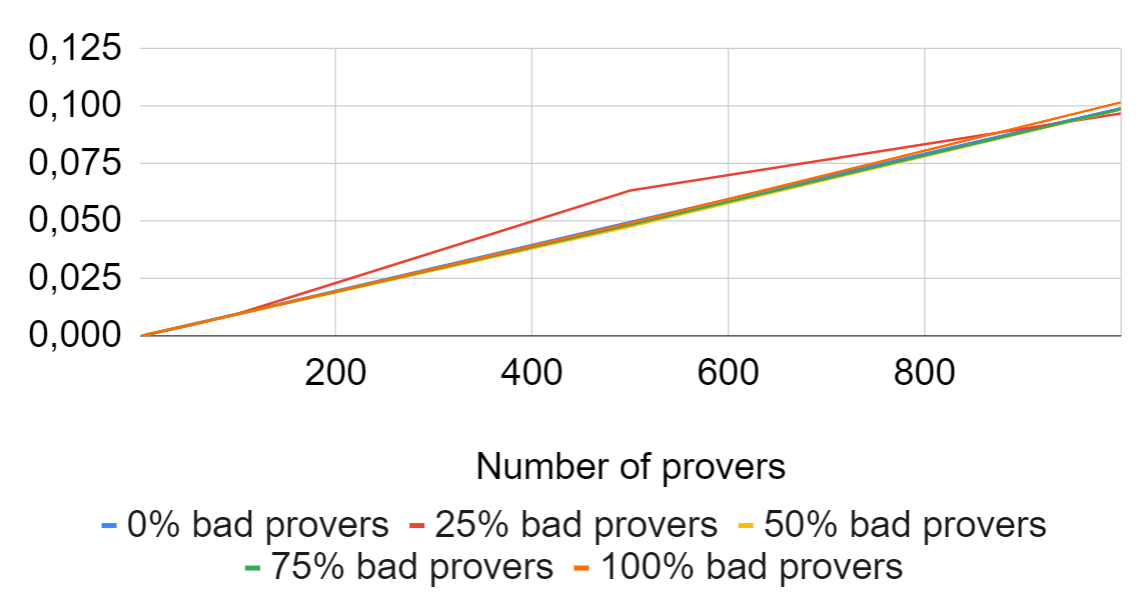
\includegraphics[width=.90\linewidth]{Images/aggregation.png}  
  \caption{Aggregation times comparison}
  \label{fig:aggregation_comparison}
\end{figure}
\begin{figure}
  \centering
  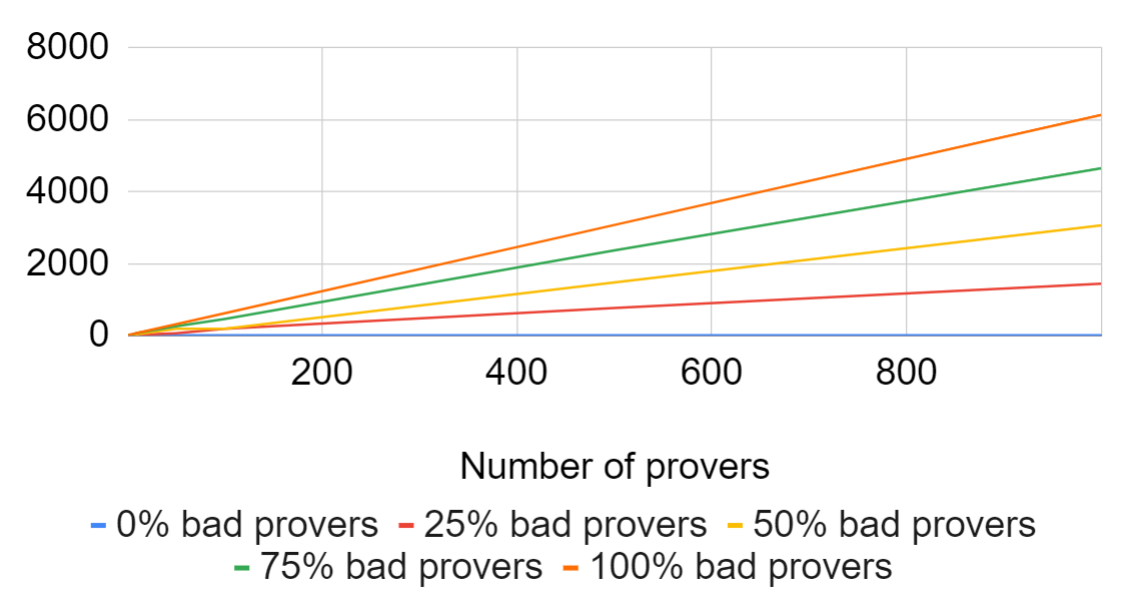
\includegraphics[width=.90\linewidth]{Images/verification.png}  
  \caption{Verification times comparison}
  \label{fig:verification_comparison}
\end{figure}
\begin{figure}
  \centering
	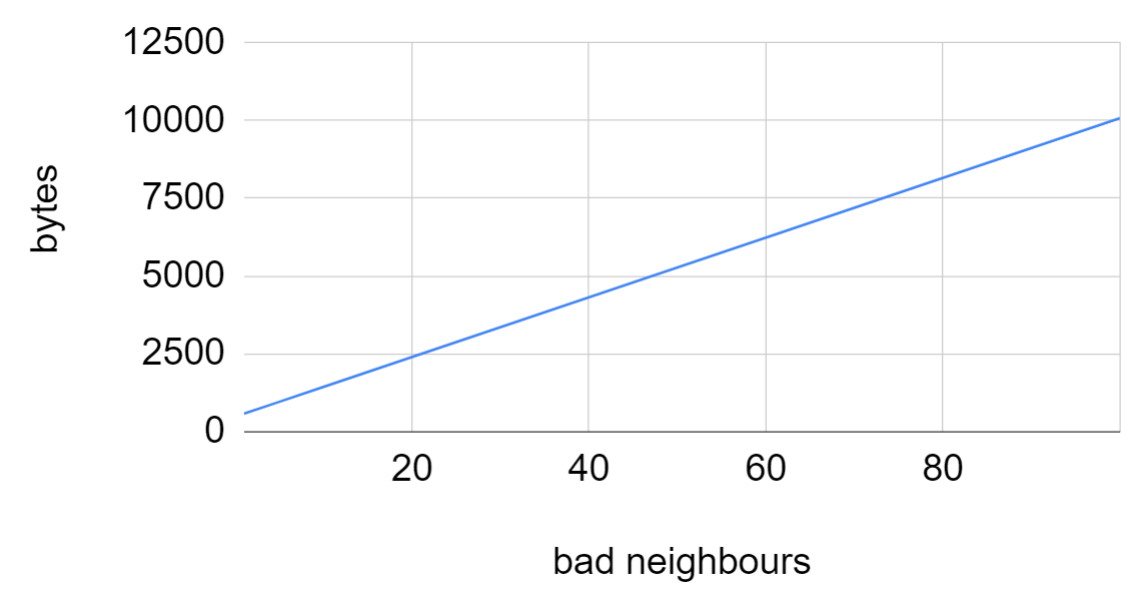
\includegraphics[width=.90\linewidth]{Images/memory_cost.png} 
	\caption{Memory cost for the aggregator} 
  \label{fig:memory_cost}
\end{figure}


\section{Conclusions}

[...]

\balance
\printbibliography[title={Bibliography}] % Print the bibliography, section title in curly brackets
\balance


\end{document}
